% This file was created by tikzplotlib v0.9.6.
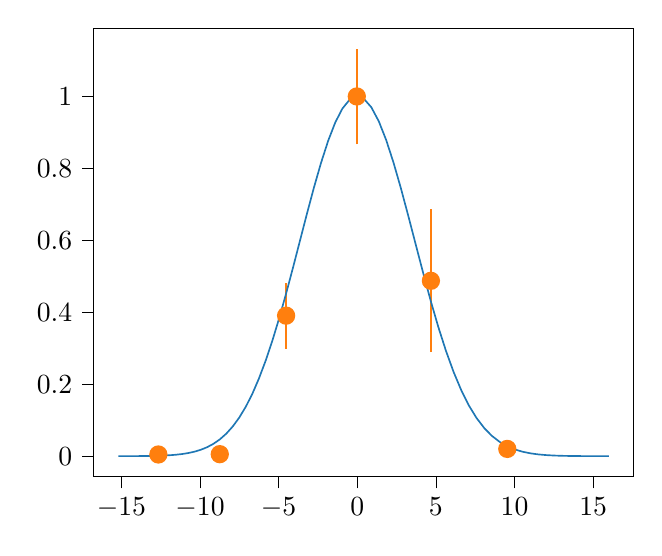
\begin{tikzpicture}

\definecolor{color0}{rgb}{1,0.498039215686275,0.0549019607843137}
\definecolor{color1}{rgb}{0.12156862745098,0.466666666666667,0.705882352941177}

\begin{axis}[
tick align=outside,
tick pos=left,
x grid style={white!69.0196078431373!black},
xmin=-16.750022610979, xmax=17.5625278205819,
xtick style={color=black},
y grid style={white!69.0196078431373!black},
ymin=-0.0566298510126379, ymax=1.18968690857077,
ytick style={color=black}
]
\path [draw=color0, semithick]
(axis cs:-4.52524479559365,0.299268820624092)
--(axis cs:-4.52524479559365,0.481932891354633);

\path [draw=color0, semithick]
(axis cs:-8.74341152865101,0.00434167178425971)
--(axis cs:-8.74341152865101,0.00672697580067228);

\path [draw=color0, semithick]
(axis cs:-12.6471499750575,0.0025631556316714)
--(axis cs:-12.6471499750575,0.00685251811732557);

\path [draw=color0, semithick]
(axis cs:4.68180096928977,0.288945057451303)
--(axis cs:4.68180096928977,0.686100268555939);

\path [draw=color0, semithick]
(axis cs:9.53786463242363,0.0123240707514649)
--(axis cs:9.53786463242363,0.028058707772011);

\path [draw=color0, semithick]
(axis cs:-0.0303111881273633,0.866963853228478)
--(axis cs:-0.0303111881273633,1.13303614677152);

\addplot [semithick, color1]
table {%
16.0028664373291 2.09107866078145e-05
15.5019804060835 4.32026966794313e-05
15.0010134446593 8.65247659168137e-05
14.5000129794234 0.00016846843599711
13.9990612616521 0.000317621566449047
13.5095902258752 0.000572652005800215
13.0089653000154 0.00102252272783255
12.508552590023 0.00177437331203595
12.0083994651273 0.00299401900027605
11.5203311831527 0.0048639818663355
11.0209718841691 0.00780234899509983
10.522031527847 0.0122177458350964
10.0356467098536 0.0184647027436416
9.53786463242363 0.0275432326616724
9.05293227613731 0.0397413362292673
8.55652691354178 0.056586017969222
8.07328410735344 0.0780965738763003
7.57848269775676 0.106443058198679
7.09715431765188 0.140853843537707
6.60416962481855 0.184135710586302
6.12499130656764 0.233971162200415
5.63408886041246 0.293369389276132
5.15728469809953 0.35847118331985
4.68180096928977 0.429962617706465
4.19445786969287 0.508495778844873
3.72169700760152 0.587599751400865
3.2504410303895 0.666830441805864
2.76716254755995 0.745785888317693
2.2989438023173 0.816833786397714
1.83238757889452 0.879465465986436
1.36756715329542 0.930973848959404
0.89050442157629 0.970138154833876
0.429152481010124 0.99298347321993
-0.0303111881273633 0.999964864660548
-0.487836802998437 0.990934601497163
-0.943377343248265 0.966493465996016
-1.39687879947519 0.927959663251433
-1.84827411185583 0.877166583706867
-2.31235747521905 0.814342168927651
-2.7595525309512 0.746139013335926
-3.20448712682099 0.673342096157743
-3.64710983931649 0.598502772271936
-4.08738073171223 0.524071220820839
-4.52524479559365 0.452105296199492
-4.96064151515727 0.38429216206419
-5.3935303935364 0.321874680850281
-5.82384575993214 0.265657644753217
-6.25154788645878 0.216130214744231
-6.66051471598014 0.174488881110224
-7.08272032371984 0.13788836740382
-7.50217143301498 0.107425330446791
-7.91880044686293 0.0825251736176341
-8.3325603241366 0.0624266731452902
-8.74341152865101 0.0465585658203397
-9.15130722291967 0.0342197077323746
-9.55620587302388 0.0247986018924741
-9.95805984926624 0.0177041465166756
-10.3396653261676 0.0126260602741104
-10.7352305835748 0.00877205506388833
-11.1276417048484 0.0060058227896583
-11.5168608429633 0.00406114067632952
-11.9028433293092 0.00270359515613201
-12.2855690608588 0.00177125330725246
-12.6471499750575 0.00116287680253254
-13.0232245202713 0.000744042815509411
-13.3959578043359 0.00046872608321309
-13.7653324428646 0.000291790653102558
-14.1313227863844 0.000178794834663396
-14.4755031362349 0.000110166381860217
-14.834642744605 6.5888373852192e-05
-15.1903612277262 3.89053007589173e-05
};
\addplot [semithick, color0, mark=*, mark size=3, mark options={solid}, only marks]
table {%
-4.52524479559365 0.390600855989362
-8.74341152865101 0.005534323792466
-12.6471499750575 0.00470783687449848
4.68180096928977 0.487522663003621
9.53786463242363 0.0201913892617379
-0.0303111881273633 1
};
\end{axis}

\end{tikzpicture}
